
%(BEGIN_QUESTION)
% Copyright 2010, Tony R. Kuphaldt, released under the Creative Commons Attribution License (v 1.0)
% This means you may do almost anything with this work of mine, so long as you give me proper credit

This pH monitoring system triggers an alarm if the pH value of the process water in the neutralization tank drifts past either of two threshold (trip) values:

$$\includegraphics[width=15.5cm]{i00239x01.eps}$$

Answer the following questions about this pH alarm system:

\vskip 10pt

\begin{itemize}
\item{} If a wire breaks loose at TB56-4, creating an ``open'' fault in the loop circuit, determine what will happen at the alarm unit (AAH, AAL-41) and also where you would expect to measure voltage in the loop circuit and where you would expect to measure {\it no} voltage in the loop circuit.
\vskip 20pt
\item{} If breaker \#25 in panel L4 suddenly trips, what will happen in this system?  Will an operator still be able to read the pH value of the water in the neutralization tank?
\vskip 20pt
\item{} If a fire breaks out near the conduit through which cable 52 runs, causing the plastic insulation around the conductors of cable 52 to melt and consequently causing those conductors to {\it short} together, what will happen in this system?  Where would you expect to measure voltage in the loop circuit, and where would you expect to measure {\it no} voltage in the loop circuit?  Where would you expect to measure current in the loop circuit, and where would you expect to measure {\it no} current in the loop circuit?
\vskip 20pt
\item{} Calculate the loop current value when the pH measures 6.8 inside the neutralization tank.
\end{itemize}



\vskip 20pt \vbox{\hrule \hbox{\strut \vrule{} {\bf Suggestions for Socratic discussion} \vrule} \hrule}

\begin{itemize}
\item{} For those who have studied pH measurement, explain why pH ``neutralization'' is an important control process in industry.
\item{} How can we tell from this diagram whether the 4-20 mA output of transmitter AIT-41 is {\it active} or {\it passive} (i.e. {\it sourcing} or {\it sinking})?
\end{itemize}

\underbar{file i00239}
%(END_QUESTION)





%(BEGIN_ANSWER)

\noindent
{\bf Partial answer:}

\begin{itemize}
\item{} If a wire breaks loose at TB56-4, creating an ``open'' fault in the loop circuit, determine what will happen at the alarm unit (AAH, AAL-41) and also where you would expect to measure voltage in the loop circuit and where you would expect to measure {\it no} voltage in the loop circuit.  {\it The AAL would trip (but not the AAH), and we would expect to measure voltage between the wires of cable 52 but not between the wires of cable 30.}
\vskip 10pt
\item{} If a fire breaks out near the conduit through which cable 52 runs, causing the conductors inside cable 52 to {\it short} together, what will happen in this system?  Where would you expect to measure voltage in the loop circuit, and where would you expect to measure {\it no} voltage in the loop circuit?  Where would you expect to measure current in the loop circuit, and where would you expect to measure {\it no} current in the loop circuit?  {\it The AAL would trip (but not the AAH), and we would expect to measure no voltage anywhere in the loop circuit.  However, we would still have current at the terminals of the AIT-41 transmitter (although no current to the right of the short).}
\end{itemize}

%(END_ANSWER)





%(BEGIN_NOTES)

\begin{itemize}
\item{} If a wire breaks loose at TB56-4, creating an ``open'' fault in the loop circuit, determine what will happen at the alarm unit (AAH, AAL-41) and also where you would expect to measure voltage in the loop circuit and where you would expect to measure {\it no} voltage in the loop circuit.  {\it The AAL would trip (but not the AAH), and we would expect to measure voltage between the wires of cable 52 but not between the wires of cable 30.}
\vskip 10pt
\item{} If breaker \#25 in panel L4 suddenly trips, what will happen in this system?  Will an operator still be able to read the pH value of the water in the neutralization tank?  {\it Both alarms would go dead, but the indicating transmitter (AIT-41) would still properly indicate pH.}
\vskip 10pt
\item{} If a fire breaks out near the conduit through which cable 52 runs, causing the conductors inside cable 52 to {\it short} together, what will happen in this system?  Where would you expect to measure voltage in the loop circuit, and where would you expect to measure {\it no} voltage in the loop circuit?  Where would you expect to measure current in the loop circuit, and where would you expect to measure {\it no} current in the loop circuit?  {\it The AAL would trip (but not the AAH), and we would expect to measure no voltage anywhere in the loop circuit.  However, we would still have current at the terminals of the AIT-41 transmitter (although no current to the right of the short).}
\vskip 10pt
\item{} If pH = 6.8, current = 11.68 mA
\end{itemize}



















\vskip 20pt \vbox{\hrule \hbox{\strut \vrule{} {\bf Virtual Troubleshooting} \vrule} \hrule}

This question is a good candidate for a ``Virtual Troubleshooting'' exercise.  Presenting the diagram to students, you first imagine in your own mind a particular fault in the system.  Then, you present one or more symptoms of that fault (something noticeable by an operator or other user of the system).  Students then propose various diagnostic tests to perform on this system to identify the nature and location of the fault, as though they were technicians trying to troubleshoot the problem.  Your job is to tell them what the result(s) would be for each of the proposed diagnostic tests, documenting those results where all the students can see.

During and after the exercise, it is good to ask students follow-up questions such as:

\begin{itemize}
\item{} What does the result of the last diagnostic test tell you about the fault?
\item{} Suppose the results of the last diagnostic test were different.  What then would that result tell you about the fault?
\item{} Is the last diagnostic test the best one we could do?
\item{} What would be the ideal order of tests, to diagnose the problem in as few steps as possible?
\end{itemize}


\vfil \eject

\noindent
{\bf Prep Quiz:}

Suppose a technician decides to break the 4-20 mA loop circuit at TB-56 to take a current measurement.  Which effect will immediately occur?

$$\includegraphics[width=15.5cm]{i00239x01.eps}$$

\begin{itemize}
\item{} The low-pH alarm will immediately activate
\vskip 5pt 
\item{} The high-pH alarm will immediately activate
\vskip 5pt 
\item{} The pH transmitter will immediately power down
\vskip 5pt 
\item{} The mixer motor will immediately shut off
\vskip 5pt 
\item{} The water's pH value will begin to rise
\vskip 5pt 
\item{} The water's pH value will begin to fall
\end{itemize}


\vfil \eject

\noindent
{\bf Prep Quiz:}

Calculate the pH value of the water inside this neutralization tank if the analyzer's output current signal is 17.5 milliamps.

$$\includegraphics[width=15.5cm]{i00239x01.eps}$$

\begin{itemize}
\item{} 12.08 pH
\vskip 5pt 
\item{} 8.44 pH
\vskip 5pt 
\item{} 10.94 pH
\vskip 5pt 
\item{} 11.69 pH
\vskip 5pt 
\item{} 10.44 pH
\vskip 5pt 
\item{} 11.44 pH
\end{itemize}


%INDEX% Basics, 4-wire self-powered transmitter: circuit analysis
%INDEX% Measurement, analytical: pH
%INDEX% Process: water pH neutralization (generic)

%(END_NOTES)

